\chapter{Results}
\label{chap:results}
The datasheet of our \ce{NdFeB} particles specifies that their residual magnetic field is \qtyrange{730}{760}{\milli\tesla}. Full saturation (\qty{>95}{\percent}) is achieved when a \qty{2}{\tesla} field is applied. Our method of magnetising the particle was limited to a \qty{1.4}{\tesla} field. As such, it is likely that we did not achieve the full saturation of the particle and that the residual magnetic field is lower than specified. Assuming a roughly linear relation between the two values, we estimate the residual magnetic field of our particles to be \qtyrange{510}{530}{\milli\tesla}. The density of the particles is given as \qty{7430}{\kilo\gram\per\cubic\meter}.

These values, together with the simulation of the magnetic field distribution in the trap, allows us to estimate the required driving frequency and the resulting eigen frequency.

\begin{figure}
    \centering
    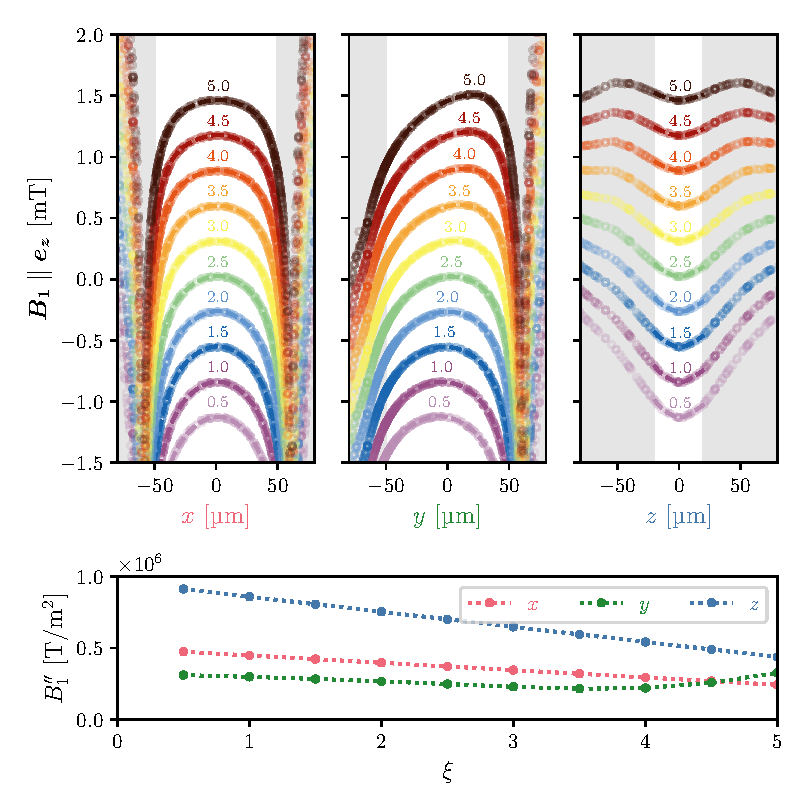
\includegraphics{figures/magnetic_field_curvature.pdf}
    \caption{the \textbf{top} figures from left to right show $z$-component of the magnetic field evaluated along a line parallel to the $x$-, $y$- and $z$-axis respectively through the origin. The gray zones indicate the boundaryies of the trap. The \textbf{bottom} figure shows the curvature of the magnetic field for these calculations evaluated in the extrema. The simulations were performed for $i_1=\qty{0.5}{\ampere}$ and $\xi$ between \numrange{-0.5}{-5}. The curves have been labelled with the corresponding value for $\xi$.}
\end{figure}

\section{Measurements at atmospheric pressure}
\label{sec:measurements-at-atmospheric-pressure}
At atmospheric pressure we determined the dependence of $\omega_{x,y}$ on $\Omega$ and $i_1$. In these measurements the ratio $\xi$ was kept constant. The spectra are obtained using the lock-in amplifier connected to the photodiode. Due to the low Q-factor at atmospheric pressure, it is not possible to tell the $x$- and $y$-modes apart. The results are shown in \autoref{fig:xy-mode-dependence-1bar}. The $z$-mode is not visible in these measurements. In addition to this the dependence of the rotational mode on $B_0$ is shown in \autoref{fig:rotational-mode-dependence-1bar}. We note three curves with a apparently linear dependence on $B_0$. The two additional curves are modulations of the resonance peak with the trapping frequency. A fourth curve can be seen in the bottom right. Its origin is unclear. A fit has not been made due to the sparsity of the data. $\omega_\alpha$ has not been observed.

\begin{figure}
    \centering
    \begin{subfigure}{0.45\textwidth}
        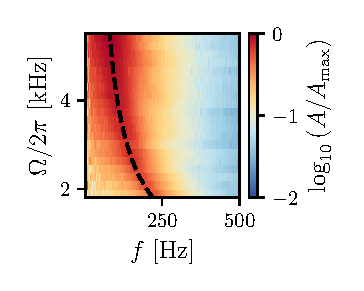
\includegraphics{figures/xy_mode_dependence_on_driving_frequency.pdf}
        %\label{fig:xy-mode-dependence-on-driving-frequency-1bar}
    \end{subfigure}
    \begin{subfigure}{0.45\textwidth}
        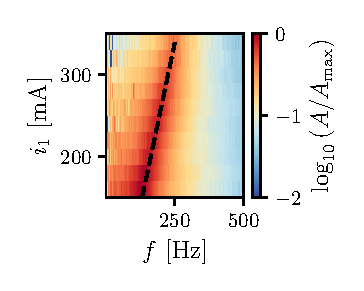
\includegraphics{figures/xy_mode_dependence_on_inner_current.pdf}
        %\label{fig:xy-mode-dependence-on-inner-current-1bar}
    \end{subfigure}
    \caption{The dependence of $\omega_{x,y}$ on $\Omega$ (\textbf{left}) and $i_1$ (\textbf{right}) at atmospheric pressure. The dashed lines are a fit following the theory of $\omega_{x,y}(\Omega) \sim 1 / \Omega$ and $\omega_{x,y}(i_1) \sim i_1$. The corresponding prefactors are $2\pi \cdot \qty{377.33170211685874\pm9.030914540546724}{\kilo\hertz\per\hertz}$ and \qty{626.5282946695123\pm20.984120764687987}{\hertz\per\ampere}. The normal value for $\Omega = 2\pi \cdot \qty{2.5}{\kilo\hertz}$ and $i_1 = \qty{200}{\milli\ampere}$ when they are not part of the sweep, the ratio $\chi = 2$ is always kept constant.}
    \label{fig:xy-mode-dependence-1bar}
\end{figure}

\begin{figure}
    \centering
    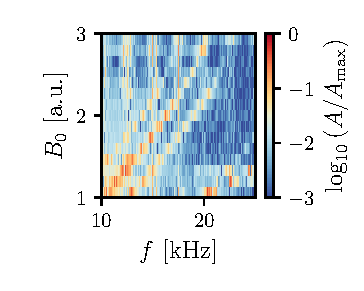
\includegraphics{figures/rotational_mode_dependence_on_B0.pdf}
    \caption{The dependence of $\omega_{\gamma,\tilde\beta}$ on $B_0$ at atmospheric pressure.}
    \label{fig:rotational-mode-dependence-1bar}
\end{figure}
